\documentclass[a4paper]{article}

\usepackage[utf8]{inputenc}
\usepackage[T1]{fontenc}
\usepackage{textcomp}
\usepackage[english]{babel}
\usepackage{amsmath, amssymb}


%figure support
\usepackage{import}
\usepackage{xifthen}
\pdfminorversion=7
\usepackage{pdfpages}
\usepackage{transparent}
\newcommand{\incfig}[1]{%
	\def\svgwidth{\columnwidth}
	\import{./figures/}{#1.pdf_tex}
}
\graphicspath{ {./figures/} }
\pdfsuppresswarningpagegroup=1

\begin{document}
	\title{EEL4768.04 Homework 6 Due 11/26/19}
	\author{Brandon Thompson 5517}
	\maketitle

	\begin{enumerate}
		\item What are interrupts?\\
			Interrupts are signals to the processor by either hardware or software that
			indicate an event needs immediate attention.
		\item How does embedded system/processor handle interrupts?
			\begin{itemize}
				\item Micro-controller stops the current instruction and saves the PC address.
				\item Saves current status of all interrupts internally (not stack).
				\item Jumps to memory location of the interrupt of vector table that holds
					the address of the interrupts service routine.
				\item Micro-controller gets the address of the ISR from the interrupt vector
					table and jumps to it. It starts to execute the interrupt service
					routine, which is RETI (return from interrupt).
				\item Upon exiting the RETI instruction, the micro-controller returns to the
					location where it was interrupted. First, it gets the program counter
					from the stack by popping the top bytes of the stack into the PC.
					Then start to execute from that address.
			\end{itemize}
		\item What are multiple interrupts?\\
			When an interrupt is triggered during another interrupt or if more than one is passed
			to the micro-controller at the same time.
		\item How does embedded systems/processor handle multiple interrupts?\\
			It would follow the above process until another interrupt is triggered, then it will
			check the priority of the each interrupt and execute the one that is ranked higher,
			then follow with the lower ranked interrupt.
		\item What is I/O interfacing?\\
			A way of connecting the outside world to a processor using a input device to gather
			info or an output device to retrieve data from the processor.
		\item How can we interface I/O device with a processor?\\
			\begin{itemize}
				\item Memory mapped I/O: Load or store can either access a memory location
					or an I/O device
					\begin{figure}[ht!]
						\centering
						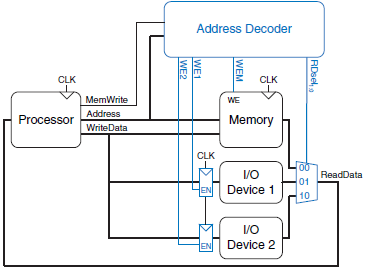
\includegraphics[width=0.8\textwidth]{mem_map_io}
						\caption{Support hardware for memory-mapped I/O.}
						\label{fig:mem_map_io}
					\end{figure}
			\end{itemize}
	\end{enumerate}
\end{document}
